\section{Hierarchical clustering}

With K-means clustering we had to predefine the number of clusters $K$. This can be a disadvantage, since we would have to do some initial analysis of the data prior. Hierarchical clustering does not require this predefinition. It uses a bottom-up or agglomerative approach to build a dendrogram starting from the observation leaves and ends up combining this into clusters at the trunk. This gives us a flexibility in the number of clusters.

\subsection{Theory}

Agglomerative states that each observation starts in its own cluster and with each iteration of the process are paired with other clusters as we move up the hierarchy.  This is based on a \textit{metric} criteria, a measure of distance between the pairs, and a \textit{linkage} criteria that indicate the dissimilarity between pairwise sets.

\noindent A common metric is Euclidean distance:

\[ \parallel a - b \parallel_{2} = \sqrt{\sum (a_{i} - b_{i})^{2}} \]
which this the straight-line distance between two points in Euclidean space (\textit{n}-space with \textit{n}-tuples of real numbers). Between two points \textit{a} and \textit{b} given by ($X_a$, $Y_a$) and ($X_b$, $Y_b$) the Euclidean distance d(a,b) is:

\[ d(a,b) = \sqrt{(X_a - X_b)^2 + (Y_a - Y_b)^2} \]


\noindent Linkage determines which distances to use between sets of observations, i.e. how they are grouped together. \textit{Single} minimizes the distance between the closest elements in clusters, \textit{complete} maximizes distance between the farthest elements, \textit{average} finds the mean of all pairwise distances, and \textit{ward} joins clusters based on the total distance between their centroids. Figure \ref{fig:linkagecriteria} shows three kinds of linkages to calculate distance.

\begin{figure}[H]
	\centering
	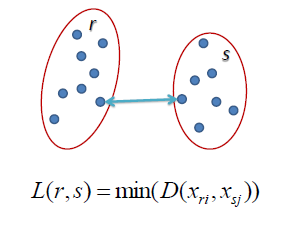
\includegraphics[width=0.3\textwidth]{clusteringMethods/hierarchicalclustering/fig/ClusteringSingle.png}
	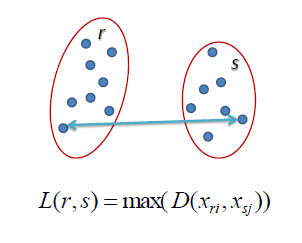
\includegraphics[width=0.3\textwidth]{clusteringMethods/hierarchicalclustering/fig/ClusteringComplete.png}
	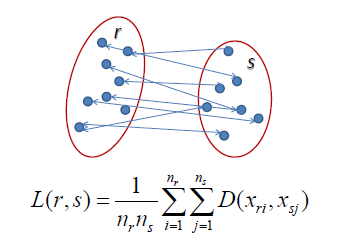
\includegraphics[width=0.3\textwidth]{clusteringMethods/hierarchicalclustering/fig/ClusteringAverage.png}
	\caption{The single,  complete and average linkage criteria.}
	\label{fig:linkagecriteria}
\end{figure}

\noindent The algorithmic steps for hierarchical clustering are:

\noindent 1. Start with \textit{N} clusters, one for each data point. \\
\noindent 2. Merge the clusters that are closest to each other. This gives \textit{N-1} clusters. \\
\noindent 3. Calculate the distance between the clusters using a linkage criteria (complete, single etc.) \\
\noindent 4. Repeat step 2 and 3 until we end up with one cluster with \textit{N} data points. The end result is a dendrogram picturing the distance (clusters) as a function of the observations (labels).

\subsection{Results}

In Lab 10.5.2 we use hierarchical clustering to group a 50 x 50 matrix of random observations using Euclidean distance and complete linkage. The AgglomerativeClustering package from Sklearn provides agglomerative clustering functionality in Python to recursively  merge pairs of clusters.

\begin{figure}[H]
	\begin{lstlisting}[caption=Performing AC in Python, label={lst:acpython}, language=Python]
		import sklearn.discriminant_analysis
		from sklearn.discriminant_analysis import QuadraticDiscriminantAnalysis
	\end{lstlisting}
\end{figure}